% mainfile: ../../../../master.tex
\subsection{Pick up samples collected during winter survey}
% The part of the label after the colon must match the file name. Otherwise,
% conditional compilation based on task labels does NOT work.
\label{task:20180305_cj0}
\tags{smp}
\authors{cj}
%\files{}
\persons{Tómas Ármann Hafsteinsson, Kristinn Guðmundsson, Mia Cerfonteyn}

According to MarineTraffic\sidenote{\url{www.marinetraffic.com}} the research vessel - Bjarni Sæmundsson - came back to Reykjavík on Sunday 4\textsuperscript{th} March at 01:00 PM (cf. figure \ref{fig:20180305_marine_traffic_bjarni}). After contacting Kristinn Guðmundsson to make sure the crew would be on board to help me with the crane, Tómas and I went to fetch the samples and Mia's personal belongings. We brought back the bottles of seawater with 1\%lugol to Matís and then we had to go back to the harbour to fetch the two liquid nitrogen tanks and bring them back to Matís.
\mistake{One of the two nitrogen has no more cap. Mia warned me about this, apparently it was damaged during the survey.}

\begin{figure}[htp] % position of the figure 
    \centering
    \caption{Screen capture showing the information about Bjarni Sædmundsson arrival and departure}
    \label{fig:20180305_marine_traffic_bjarni}
    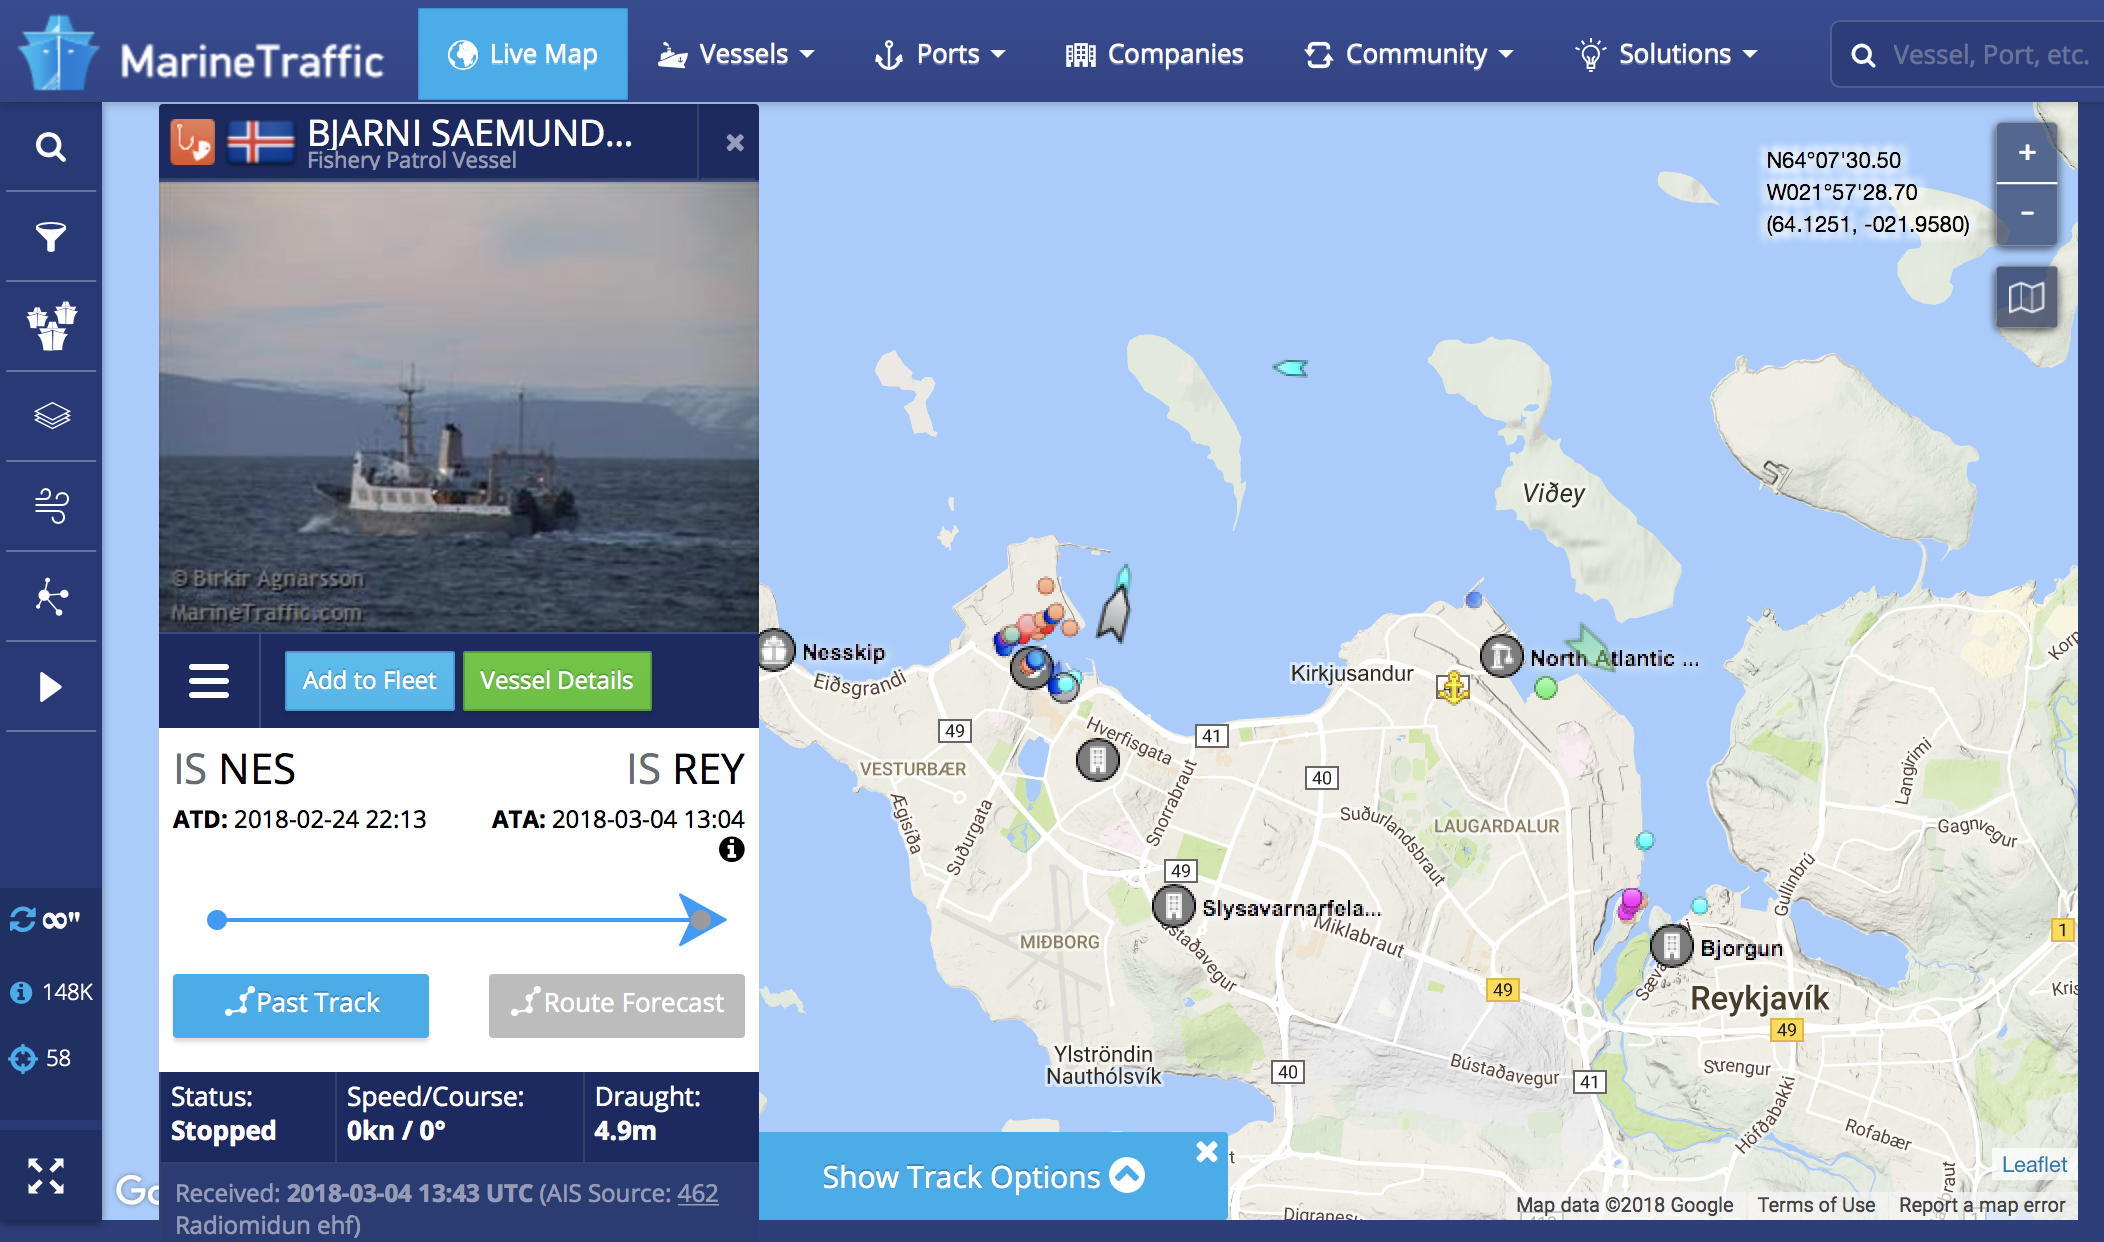
\includegraphics[width=\textwidth]{graphics/screenshots/20180305_marine_traffic_bjarni.png}
\end{figure}